\documentclass[12pt,a4,english,finnish,pdflatex%,handout
]{beamer}
\definecolor{MyGreen}{RGB}{50, 120, 50}
\usecolortheme[named=MyGreen]{structure}

\usepackage{babel}
\usepackage[utf8]{inputenc}
\usepackage[T1]{fontenc}
\usepackage{amsmath,amssymb} 
\usepackage{animate}
\usepackage{multimedia}

\usepackage{natbib}
\bibpunct[: ]{(}{)}{,}{}{}{;}

\usepackage{tikz}

\usepackage{tipa}

\usepackage{hyperref}

\setbeamertemplate{navigation symbols}{}

\graphicspath{{figures/}}

\setlength{\leftmargini}{0pt}
\setlength{\leftmarginii}{1em}

\newcommand{\kommentti}[1]{
  {\bf[#1]}
}



\begin{document}
\title{Ideas for Fantastic ((un)real) Speech} 
\author{Pertti Palo} 
\date{17 April 2022}

\frame{\titlepage
} 

\frame{\frametitle{Land acknowledgement}
We wish to acknowledge and honor the Miami, Delaware, Potawatomi, Kickapoo, and
Shawnee people, on whose ancestral homelands we are today and/or on whose
ancestral homelands I have worked on this presentation. 
}

\frame{\frametitle{Housekeeping and Warnings}
  \begin{itemize}
  \item I want to keep this a safe space of mutual respect.
  \item The organisers told me that I should tell you, that I will swear during
  this presentation.
  \item Personally, I find it more important to give you a content warning
  concerning topics such as colonization, oppression, pejoratives, etc. which
  may or may not come up depending on where the conversation takes us.
  \end{itemize}  

  \vspace*{.5cm}

  \begin{itemize}
    \item Please feel free to ask questions at any point.
    \item There will also be time for discussion and questions afterwards. I do
    not intend to fill the full hour with just me talking.
  \end{itemize}
}


\frame{\frametitle{Outline}
  \begin{itemize}
  \item {\usebeamercolor[gray]{} Yesterday: Borrowing a Language 101}
  \item  Today: Ideas for Fantastic ((un)real) Speech
    \begin{itemize}
      \item Housekeeping and warnings
      \item Who am I and why am I here?
      \item Dragons and Bird people
      \item Speech and magic
      \item Some food for thought
    \end{itemize}
  \end{itemize}
}

\frame{\frametitle{Who's this guy?}
  \begin{columns}
    \begin{column}{5cm}
      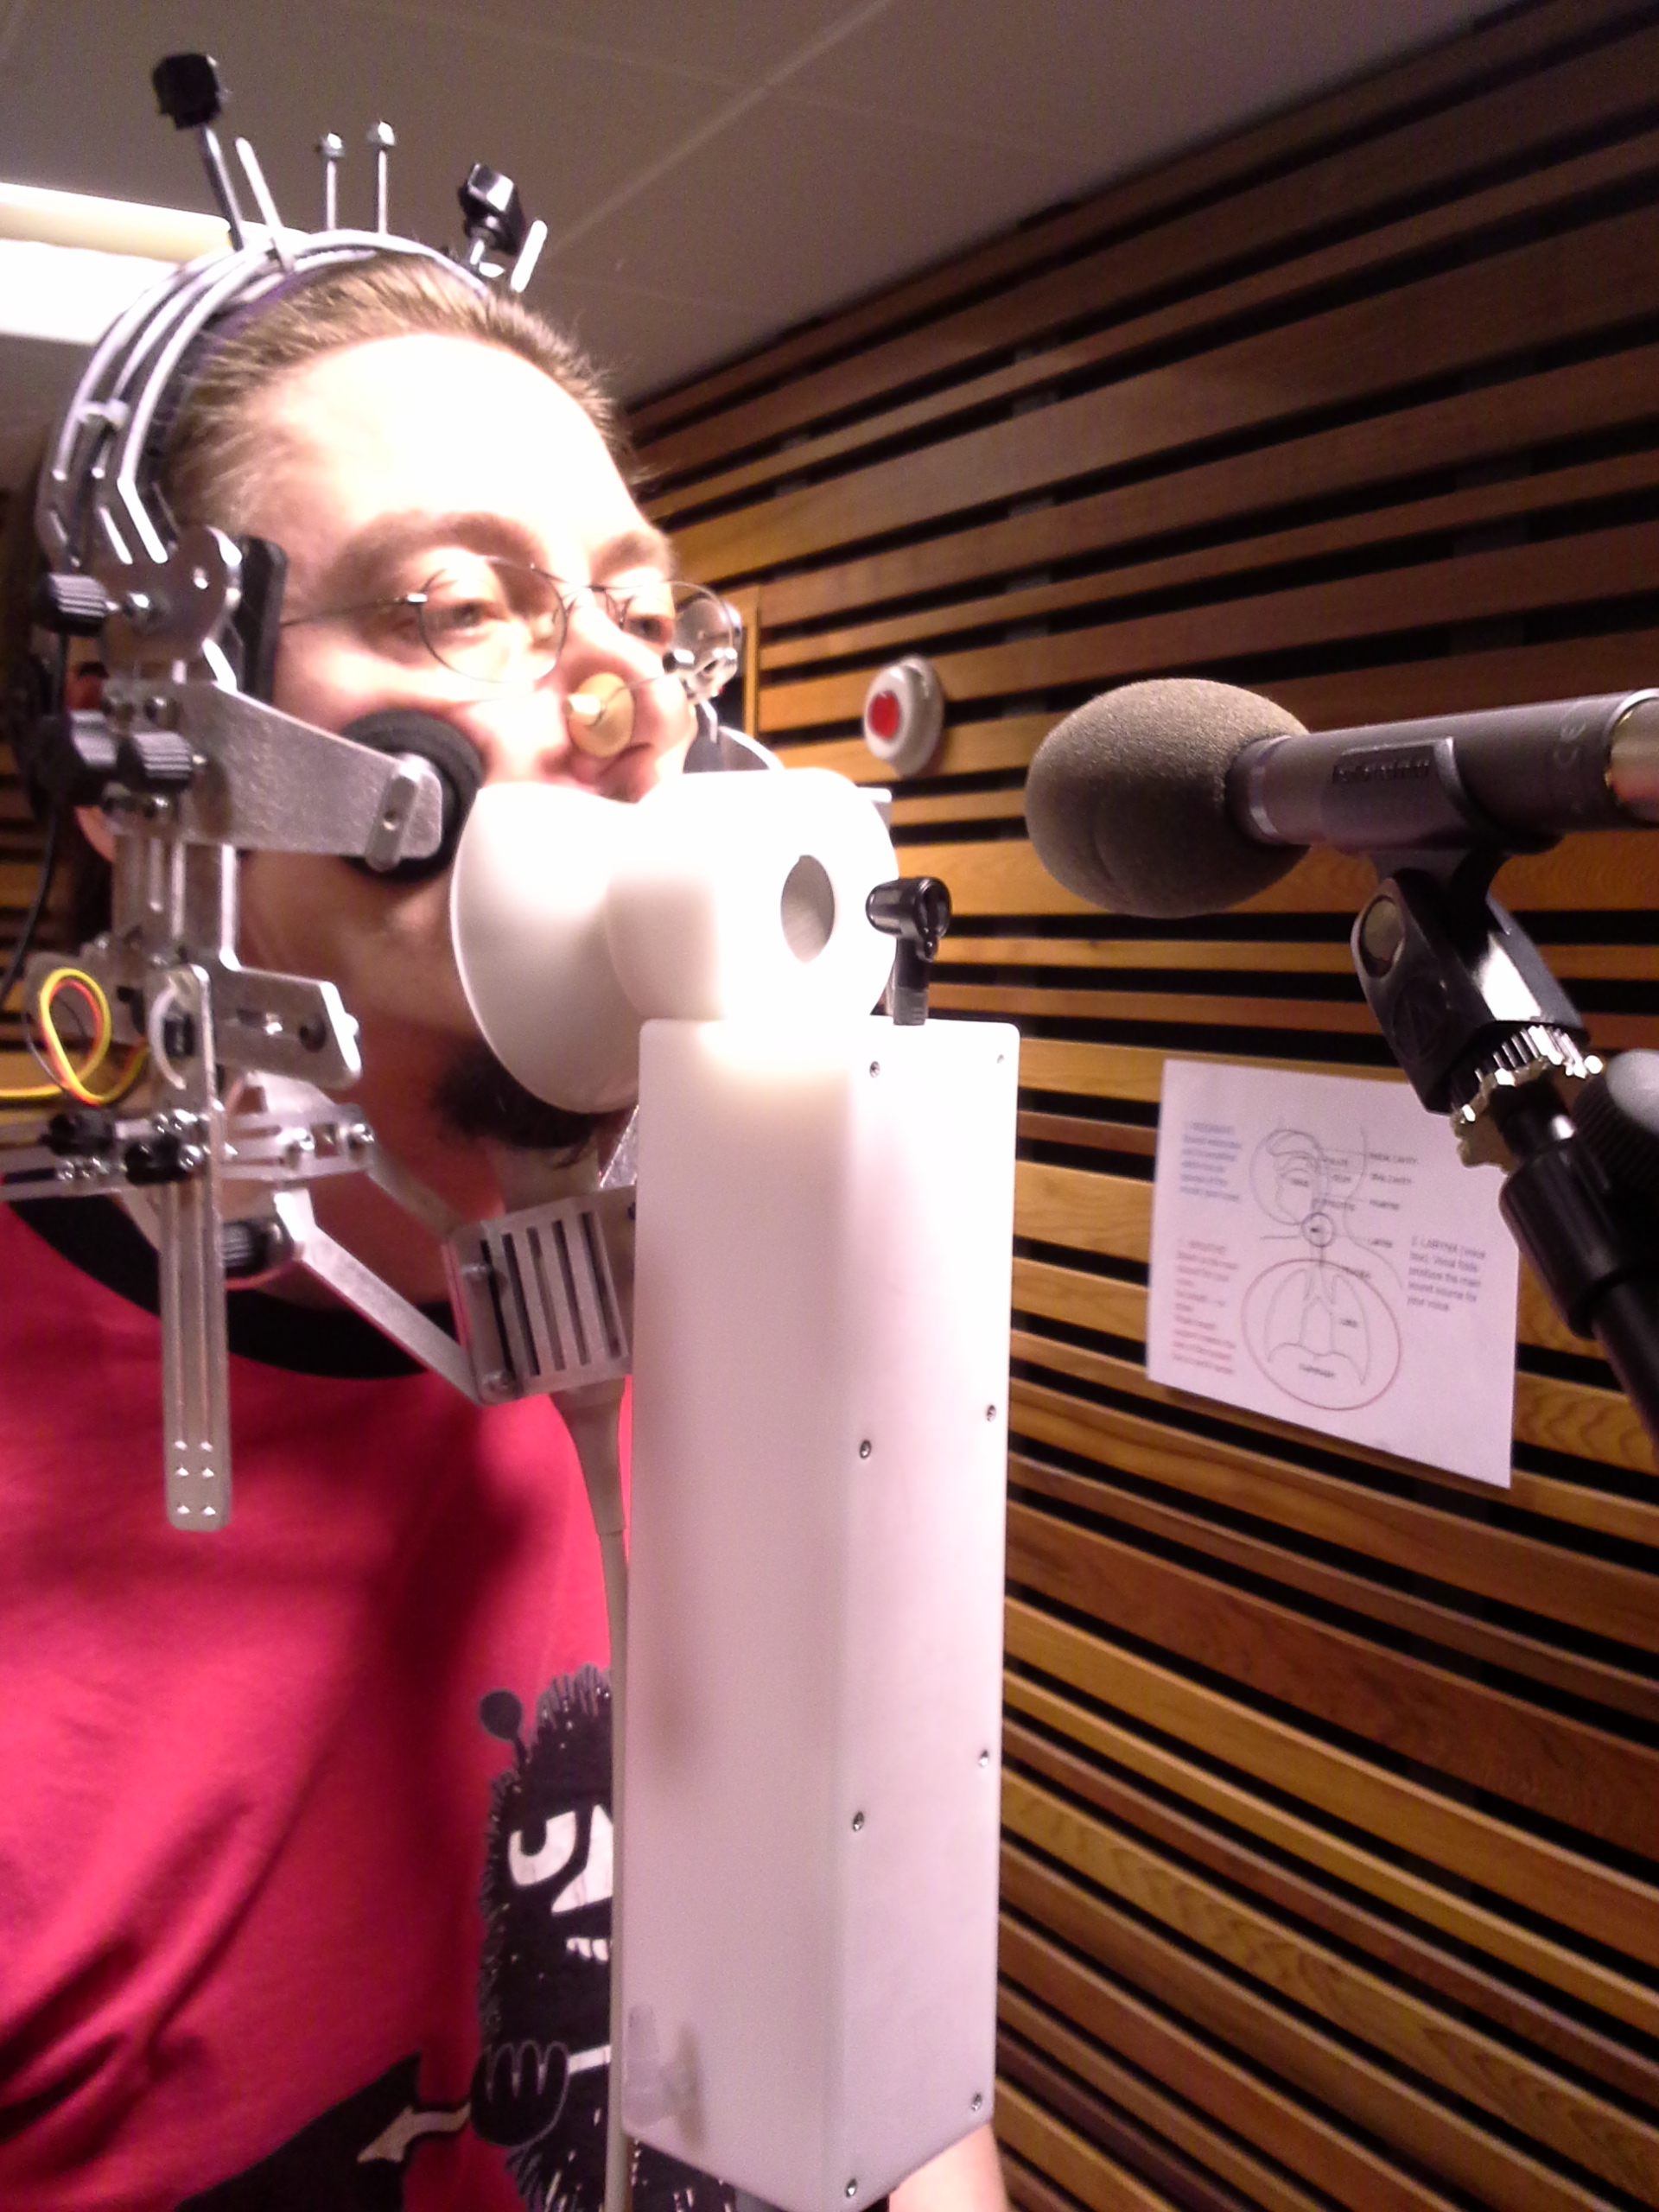
\includegraphics[width=\columnwidth]{uti_eva.png}
    \end{column}
    \begin{column}{5cm}
      \begin{itemize}
      \item Pertti Palo
      \item I've got a couple of degrees loosely speaking in engineering.
      \item I've also got a PhD in Phonetics.
      \item I have obviously not ever collected articulatory data on a live
      dragon, but I have spent a lot of time learning how to think about speech
      production and articulation.
      \end{itemize}
    \end{column}
  \end{columns}
} 

\frame{\frametitle{What lead me here?}
\begin{itemize}
  \item I can no longer tell if LotR or interest in speech and language came
  first in my life.
  \item I am not a text linguist but rather a phonetician and a speech
  researcher.
  \item Besides a speech researcher with 20+ years of experience, I've been an
  RPG enthusiast for 30+ years. 
  \item Recently I've also started training as an oral storyteller which has
  some interesting connections with RPGs but also with science.
\end{itemize}
}

\frame{
\centering
\vfill
Dragons and bird people
\vfill
}

\frame{\frametitle{Dragon speech: Let's first talk about humans}

\begin{itemize}
  \item Have you ever considered how humans produce speech?
\end{itemize}

\includegraphics[width=.49\textwidth]{Places_of_articulation.svg.png}
\includegraphics[width=.49\textwidth]{DA_oe_hampaat_lisatty.jpg}

Picture on the left by user ish shwar on Wikipedia (CC BY-SA 3.0), picture on
the right by me (CC BY-SA 3.0) 
}

\frame{\frametitle{Dragon anatomy}
\begin{itemize}
  \item Have you ever considered how a huge thing like a dragon -- let's say
  Smaug -- could sound like a human?
  \item Smaug is a lot larger than a human with wildly
  different neck and mouth anatomy.
\end{itemize}

  {
    \centering
    \includegraphics[width=.75\textwidth]{Smaug_par_David_Demaret.jpg}
  }

  Picture by David Demaret via Wikipedia (CC BY-SA 3.0).
}

\frame{\frametitle{Maybe dragons are voice actors?}
\begin{itemize}
  \item Mouth is still too large,
  \item but like Colette told us in the previous panel you can alter that with
  the tongue.
\end{itemize}

  {
    \centering
    \includegraphics[width=.75\textwidth]{smaug.jpeg}
  }

  Picture by Prof Steven Lulich via my phone (CC BY-SA 3.0).

}

\frame{
\centering
\vfill
If not voice actors what then?
\vfill
}

\frame{\frametitle{Maybe mind speech?}
\begin{itemize}
  \item Maybe it's mind speech? But how's that produced and what are the rules?
  \begin{itemize}
    \item Is the range sight only?
    \item Or something like regular sound carrying distance?
    \item Is it actually illusion?
    \item Or 'just' a magic spell-like ability to produce sound at will? In
    which case a dragon could potentially produce any sound.
  \end{itemize}
  \item Even if it is mind speech how about the roar?
\end{itemize}
}

\frame{\frametitle{But maybe it's acoustic speech?}
\begin{itemize}
  \item Maybe it is acoustic speech after all but just not produced by the same
  system they use for breathing and eating?
  \begin{itemize}
    \item So what is this organ like?
    \item Something like whale sonar?
    \item Some magical thing that lives in the dragon's mouth?
  \end{itemize}
\end{itemize}
}

\frame{\frametitle{Bird people}
\begin{itemize}
  \item Have you ever considered how a small thing like a parrot can sound like
  a human?
  \item Birds don't have the same vocal anatomy as humans do. 
\end{itemize}

  {
    \centering
    \includegraphics[width=.35\textwidth]{Syrinx.jpg}
  }

  Picture by Uwe Gille via Wikipedia (CC BY-SA 3.0).
}

\frame{
\centering
\vfill
Speech and magic
\vfill
}

\frame{\frametitle{Speech and magical power in the real world: Swearing}
\begin{itemize}
  \item A lot of swear words are taboo because they are perceived as curses or
  perceived to evoke power: Damn, hell, helvetti, perkele and so many more.
  \item So are words magical? How? Why? And what consequences would this have?
  \begin{itemize}
    \item Do they need to be spoken to become magic?
    \item Power of true names: How exact do you need to be?
    \item Would a translation of a magic name do?
    \item Is rythm important internally or externally? Is the rythm relevant to
    only mages but not to non-mages?
    \item Is breath control the key to magic?
  \end{itemize}
	\item And just randomly: How about magic being tied to something that needs to
	be artificially embedded in your vocal tract?
\end{itemize}
}

\frame{
\centering
\vfill
Some food for thought
\vfill
}

\frame{\frametitle{Topics that are interesting and require care}
\begin{itemize}
  \item Speech and language minorities:
  \begin{itemize}
    \item Minority languages
    \item Prestige and non-prestige accents
  \end{itemize}
	\item impairments, social challenges, and shibboleths that don't really matter
	in intelligibility
  \begin{itemize}
    \item Stuttering
    \item Finnish /r/
  \end{itemize} 
\end{itemize}
}

\frame{\frametitle{Some ideas to play around with}
\begin{itemize}
  \item Whistled languages, languages spoken with musical instruments
  \item All the different ways of conveying meaning: tone, vowels, consonants,
  voice quality which leads to:
  \item 'Weird' sounds -- sounds that are less common (in English):
  \begin{itemize}
      \item Kargyraa, khöömei, European overtone singing 
      \item clicks, and generally the whole of what IPA covers these days, let
      alone what X-IPA covers
  \end{itemize}
  \item Synthesised voices in sci-fi and why not fantasy too.
\end{itemize}
}

\frame{\frametitle{Keeping it all together}
\begin{itemize}
  \item Don't go over the top.
  \item Use things that make sense to you, which also have a role in the story.
  \item The role maybe one of creating atmosphere but can also be something more
  involved.
  \item Humans are very curious. It is easy to make things attractive to us by
  including a partial or open ended description of something. Speaking of which:
\end{itemize}
}

\frame{\frametitle{More interesting stuff to embed in a setting}
\begin{itemize}
  \item Music
  \item Song
  \item Mouth Music
  \begin{itemize}
    \item Imitating instruments
    \item Imitating animal sounds
  \end{itemize}
\end{itemize}
}

\frame{
\centering
Thank you!\\
~\\
Let's talk!

}

\frame{\frametitle{Acknowledgements}

\begin{itemize}
  \item Again, the people who's ancestral land we are on.
  \item Wikipedia.
  \item All the good folk mentioned in passing and whose pictures I've borrowed.
  \item Copyrighted work remains the property of the legal copyright holders.
  \end{itemize}
}

\end{document}

